% cordillera-climate.tex
% ----------------------------------------------------------------------

% Copernicus manuscript
\documentclass[tc, ms]{copernicus}

% Copernicus final print
%\documentclass[tc]{copernicus}

% Copernicus discussion paper
%\documentclass[tcd, hvmath]{copernicus_discussions}

% Copernicus-like latex2rtf compatible
%% copernicus_rtf.tex
% ------------------

% Base class and packages
\documentclass{article}
\usepackage{color}
\usepackage{geometry}
\usepackage{graphicx}
\usepackage{setspace}
\onehalfspacing

% Replacements for bibtex commands
\newcommand{\citep}[1]{(\textcolor{blue}{#1})}
\newcommand{\citet}[1]{\textcolor{blue}{#1}}

% Replacements for Copernicus commands
\newcommand{\introduction}[0]{\section{Introduction}}
\newcommand{\conclusions}[0]{\section{Conclusions}}
\newcommand{\tophline}[0]{\hline}
\newcommand{\middlehline}[0]{\hline}
\newcommand{\bottomhline}[0]{\hline}
\newcommand{\unit}[1]{\ensuremath{\mathrm{#1}}}
\newcommand{\degree}[0]{\ensuremath{^{\circ}}}

% Ignore other Copernicus commands
\newcommand{\runningtitle}[1]{}
\newcommand{\runningauthor}[1]{}
\newcommand{\received}[1]{}
\newcommand{\correspondence}[1]{}
\newcommand{\pubdiscuss}[1]{}
\newcommand{\revised}[1]{}
\newcommand{\accepted}[1]{}
\newcommand{\published}[1]{}



% Coloured hyperlinks
\usepackage[colorlinks,citecolor=blue]{hyperref}

% Recognize utf-8 special characters
\usepackage[T1]{fontenc}
\usepackage[utf8]{inputenc}

% Set figures repository
\graphicspath{{figures/}}

% ----------------------------------------------------------------------
\begin{document}
% ----------------------------------------------------------------------

% Title
\title{The effect of climate forcing on numerical simulations of the Cordilleran Ice Sheet at the Last Glacial Maximum}
\runningtitle{Climate forcing for Cordilleran ice sheet simulations}

% Authors
\author[1]{Julien Seguinot}
\author[2]{Constantine Khroulev}
\author[3]{Irina Rogozhina}
\author[1]{Arjen P. Stroeven}
\author[1]{Qiong Zhang}
\runningauthor{J. Seguinot et al.}
\correspondence{J. Seguinot\\ (julien.seguinot@natgeo.su.se)}

% Affiliations
\affil[1]{Department of Physical Geography and Quaternary Geology, Stockholm University, Stockholm, Sweden}
\affil[2]{Geophysical Institute, University of Alaska Fairbanks, Fairbanks, AK, USA}
\affil[3]{Helmholtz Centre Potsdam, GFZ German Research Centre for Geosciences, Potsdam, Germany}

% For Copernicus
\received{}
\pubdiscuss{}
\revised{}
\accepted{}
\published{}

% Title
\maketitle

% Sections
% section/abstract.tex
% ----------------------------------------------------------------------

\begin{abstract}
We present an ensemble of numerical simulations of the Cordilleran Ice Sheet during the Last Glacial Maximum performed with the Parallel Ice Sheet Model (PISM), using temperature offsets from present-day climatologies from five different datasets. Monthly mean surface air temperature and precipitation from the NCEP/NCAR reanalysis, the Climate Forecast System Reanalysis, the ERA-Interim reanalysis and the North American Regional Reanalysis are used to compute surface mass balance by using a positive degree-day model. Modelled ice sheet outlines and volumes appear highly sensitive to the choice of climate forcing. We assess model performance against a reconstruction of the ice margin at the Last Glacial Maximum in continental regions of northern Yukon Territory and interior Alaska. The best match between model output and the reconstructed ice margin is obtained using the North American Regional Reanalysis, which is a regional climate reanalysis with the highest resolution.
\irina{Maybe more on conclusions.}
\end{abstract}


% ----------------------------------------------------------------------
\introduction
\label{sec:intro}
% ----------------------------------------------------------------------

At the Last Glacial Maximum (LGM), glaciers of a size comparable to the present Greenland and Antarctic ice sheets covered parts of Northern America (Laurentide, Cordilleran and Innuitian ice sheets) and Northern Eurasia (Fennoscandian Ice Sheet). Numerical modelling of these former ice masses allows for a comparison between glaciological theories embedded in the models and geomorphological traces underpinning palaeo-glaciological reconstructions. Yet, a major obstacle in this exercise resides in large uncertainties concerning climate forcing, typically temperature and precipitation data, needed by numerical glacier models \citep{hebeler-etal-2008}. This includes uncertainty in representation of Earth's present climate in regions of poor station coverage, and even larger uncertainty concerning accurate reconstructions of past climate change.

Arguably the most physically sound way to force an ice sheet model in the past is to couple it with a General Circulation Model (GCM) \citep{yoshimori-etal-2001,calov-etal-2002,abeouchi-etal-2007,charbit-etal-2013}. However the computational demand of GCMs is such that only models of intermediate complexity can run on the time-scales of tens of thousands of years characteristic of ice sheet growth and decay.

%Irina  I think it would be reasonable to discuss the limitations of GCM in this context

Climatologies obtained from uncoupled GCM palaeo-climate simulations such as produced within the PMIP project \citep{joussaume-taylor-1995} provide a more accurate representation of past climate and are commonly used to force ice sheet models. Because they are only available for specific periods of time, they require either an assumption of steady-state \citep{huybrechts-tsiobbel-1996}, or interpolation through time between climatologies from different periods, which can be linear \citep{charbit-etal-2002}, or modulated by a ``glacial index'' weighting function derived from ice core $\delta^{18}$\,O records \citep{marshall-clarke-1999,tarasov-peltier-2004,zweck-huybrechts-2005,gregoire-etal-2012}. An important drawback in this approach is that palaeo-climate simulations themselves rely on global ice sheet reconstructions such as the ICE-4G \citep{peltier-1994} for their surface topographic boundary condition. This indirectly controls subsequently modelled ice sheet geometries, whose spatial extent tend to conform to these reconstructions.
\julien[noline]{Should this literature list be extended to studies not covering North America?}

The other side of the coin is that avoiding this circular dependence unfortunately goes hand-in-hand with a need for simplifying assumptions on Earth's past climate. They include energy balance modelling approaches \citep{tarasov-peltier-1997} and geographic parametrizations of surface mass balance \citep{robert-1991} or climate forcing \citep{johnson-fastook-2002}. Standing on a middle ground, temperature offset methods \citep{greve-etal-1999,bintanja-etal-2005} make use of the high level of detail available in present climate datasets such as gridded observation datasets, GCM output or reanalyses, while using simplifying representations of past climate deviations from this present state.

Here, we propose to address some of the uncertainties concerning climate forcing of numerical glacier models by evaluating their response, in terms of glacier extent, to inputs from several climate datasets. Few studies of this kind are presently available. \citet{quiquet-etal-2012} assessed the sensitivity of a Greenland ice sheet model to various atmospheric forcing, including a regional parametrization \citep{fausto-etal-2009}, output from several GCMs and a climate reanalysis. \citet{rodgers-etal-2004,charbit-etal-2007} tested the sensitivity of a model of the Northern Hemisphere ice sheets to different PMIP LGM simulations. Here, to limit degrees of freedom in our model, and obtain results independent from palaeo-ice sheet reconstructions such as the ICE-4G, we use a simple temperature offset approach similar to \citep{greve-etal-1999,bintanja-etal-2005} and assess ice sheet model sensitivity to the choice of present-day climate data. Rather than using GCM output, we force our model with climate reanalysis data, which include observational information through data assimilation \citep{bengtsson-etal-2007}. Furthermore, we focus our study regionally to the former Cordilleran Ice Sheet in Northern America.

\begin{figure}[t]
	\vspace*{2mm}
	\begin{center}
		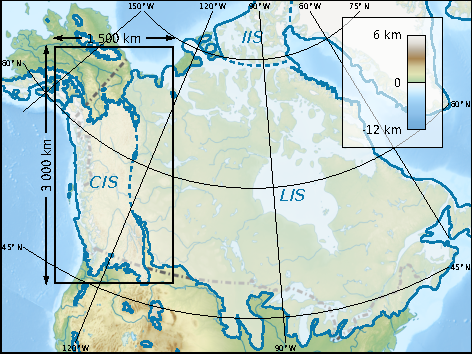
\includegraphics[width=8cm]{cordillera-climate-locmap}
	\end{center}
	\caption{Shaded relief map of northern North America. The frame delimits this study's modelling domain. The outlines of the former ice sheets depict ice cover at 14\,$^{14}$C\,ka\,BP (16.8\,cal\,ka\,BP) after \citet{dyke-2004}. The background map was made with ETOPO1 \citep{data:etopo1} and Natural Earth Data \citep{data:naturalearth}.}
	\label{fig:locmap}
\end{figure}

The Cordilleran Ice Sheet (Fig.~\ref{fig:locmap}) covered an area that presently experiences strong regional variations in climate. In a numerical modelling perspective, it is one of the least studied palaeo-ice sheets of the Northern Hemisphere, despite the fact that significant geomorphological data is available to constrain its extent \citep{jackson-clague-1991,dukrodkin-1999,kaufman-manley-2004,kleman-etal-2010,margold-etal-2011}. Although the Cordilleran Ice Sheet was not the primary target of these simulations, it has previously been modelled as part of efforts to model ice sheets in North America \citep{marshall-clarke-1999,calov-etal-2002,tarasov-peltier-1997,tarasov-peltier-2004,gregoire-etal-2012}, the Northern Hemisphere \citep{huybrechts-tsiobbel-1996,greve-etal-1999,charbit-etal-2002,charbit-etal-2007,charbit-etal-2013,johnson-fastook-2002,rodgers-etal-2004,bintanja-etal-2005,zweck-huybrechts-2005,abeouchi-etal-2007} or world-wide \citep{yoshimori-etal-2001}. While these studies reproduce the magnitude of North American glaciation at the Last Glacial Maximum (LGM) reasonably well, there exist a tendency in simulations independent from ice sheet reconstructions such as the ICE-4G to predict excessive ice cover in parts of northern Yukon Territory and continental Alaska that have remained ice-free throughout the Pleistocene \citep{dukrodkin-1999,kaufman-manley-2004}.

Here we use a Parallel Ice Sheet Model \citep[PISM,][]{web:pism} \julien{Recommended by \url{http://www.pism-docs.org/wiki/doku.php?id=citing_pism}} to simulate the extent and thickness of Cordilleran Ice Sheet at the LGM. We force our model with multiple climate datasets and compare our results to the mapped LGM ice sheet margin from \citet{dyke-2004}. To our knowledge, this is the first modelling study which specifically focus on the Cordilleran Ice Sheet since the one by \citet{robert-1991}. While \citet{robert-1991} modelling domain covered only the southern part of the ice sheet, our model also includes higher resolution and an improved treatment of ice thermodynamics and bedrock response due to large advances made in ice sheet modelling since then. Model set-up is presented in section~\ref{sec:model} and climate forcing in section~\ref{sec:climate}. Results are exposed in section~\ref{sec:results} and discussed in section~\ref{sec:discussion}.

% sections/model.tex
% ----------------------------------------------------------------------
\section{Model setup}
\label{sec:model}
% ----------------------------------------------------------------------

We use PISM, a Parallel Ice Sheet Model, version stable~0.5.12 (e.g.,) \citep{bueler-brown-2009,winkelmann-etal-2011,aschwanden-etal-2012,web:pism}. Given basal topography\irina{geothermal heat flux and sea level} and climate forcing, the model computes the thermal and dynamic state of an ice sheet and the associated lithospheric response. Our modelling domain encompasses most of the area covered by the Cordilleran Ice Sheet at LGM except from the western Alaskan ranges and includes non-glaciated regions in northern Yukon Territory and interior Alaska. Our simulations are performed in parallel on 32 cores at the Swedish National Supercomputing Center.

\subsection{Ice thermodynamics}

The Shallow Shelf Approximation (SSA) is used as a ``sliding law'' for the Shallow Ice Approximation (SIA) \citep{winkelmann-etal-2011}. SIA and SSA velocities are computed by finite difference methods on a 10\,km-resolution horizontal grid of 300 by 150 points (the modelling domain). Ice softness depends on temperature and water content through an enthalpy formulation \citep{aschwanden-blatter-2009,aschwanden-etal-2012}. Enthalpy is computed in three dimensions in up to 51 irregularly spaced layers in ice, and temperature is further computed in 11 regularly spaced layers in bedrock. A uniform geothermal heat flux of 70\,\unit{W\,m^{-2}} provides the lower boundary condition to the bedrock thermal model, and surface air temperature from the climate forcing provides the upper boundary condition to the ice enthalpy model.

A pseudo-plastic sliding law \citep{aschwanden-etal-2013} (supplement) relates the bed-parallel shear stress and the sliding velocity. The yield stress is modelled using the Mohr-Coulomb criterion. The till friction angle $\phi$ varies from 10 to 30\degree\ and is a function of contemporary bed elevation, with lowest values occurring at low elevations,
\julien{phi is independent from basal water which is computed by the model (and sliding depends on both) so the 10 to 30 degree range is meant to reflect different bedrock/sediment surfaces rather than dry vs wet beds.}

\begin{equation}
	\phi = \left\{\begin{array}{llrll}
		10      & \mathrm{for} &      &z&<  0 \\
		z/10+10 & \mathrm{for} &   0 <&z&<200 \\
		30      & \mathrm{for} & 200 <&z&     \\
	\end{array}\right.
\end{equation}

where $\phi$ is given in degrees and $z$ in meters above contemporary sea level. This models weakening of the till associated with the presence of marine sediments \citep{martin-etal-2011,aschwanden-etal-2013}. Basal topography (Fig.~\ref{fig:topo}) is derived from the ETOPO1 combined topography and bathymetry dataset \citep{data:etopo1}.\julien{NaturalEarth data are vectors (coastline, rivers, etc.) used in Fig. 1, not model input.} Sea level is lowered by 120\,m and basal topography responds to ice load following a regional isostasy model that includes lithospheric flexure and mantle relaxation \citep{lingle-clark-1985}.

% ----------------------------------------------------------------------

\subsection{Surface mass-balance}

Ice surface accumulation and ablation are computed from monthly mean surface air temperature and monthly precipitation by a temperature-index (positive degree-day) model \citep{hock-2003}. Ice accumulation is equal to precipitation when temperature is below 0\,\unit{\degree C}, and decreases to zero linearly with temperature between 0 and 2\,\unit{\degree C}. Ice ablation is computed from the number of positive degree-days, defined as the integral of temperatures above 0\,\unit{\degree C} in one year. 

The positive degree-day integral \citep{calov-greve-2005} is numerically approximated using week-long sub-intervals. It accounts for temperature variability assuming a normal distribution along a central (input) value. The temperature standard deviation is a constant model parameter and was assigned a value of 3.07\,\unit{\degree C}, which corresponds to the summer (JJA) mean, model domain-averaged monthly standard deviation of daily mean temperature from monthly mean temperature, as computed from North American Regional Reanalysis data \citep{data:narr} in a manner similar to \citet{seguinot-inreview}. The ablation model incorporates degree-day factors of 3.04\,\unit{mm\,K^{-1}\,day^{-1}} for snow and 4.59\,\unit{mm\,K^{-1}\,day^{-1}} for ice, as derived from mass-balance measurements on contemporary glaciers from the Coast Mountains and Rocky Mountains in British Columbia \citep{shea-etal-2009}.

% ----------------------------------------------------------------------

\subsection{Atmospheric corrections}

Prior to surface mass balance computation, the model dynamically applies a lapse-rate correction to surface air temperature. This correction accounts for evolution of ice thickness on the one hand, and differences between the climate forcing reference topography and the ice flow model basal topography on the other hand. It uses a reference topography distinct from the modelled basal topography and specific to each climate forcing dataset (Fig.~\ref{fig:topo}). An annual lapse-rate of 6\,\unit{\degree C\,km^{-1}} is used in all simulations. No lapse-rate corrections apply to precipitation.

As we aim to model glacial inception and growth of the Cordilleran Ice Sheet towards a configuration as last attained during the LGM, we mimic palaeo-climatic conditions by applying constant temperature offsets homogeneously over the modelling domain. Each simulation starts from ice-free conditions and runs for 10\,kyr, a time interval representative of the rapid build-up of the last Cordilleran Ice Sheet from nearly ice-free to full glacial conditions \citep{clague-1989,stroeven-etal-2010}.

% sections/climate.tex
% ----------------------------------------------------------------------
\section{Climate forcing}
\label{sec:climate}
% ----------------------------------------------------------------------

Our atmospheric forcing consists of monthly climatologies of surface air temperature and precipitation obtained from one observational dataset, three global reanalyses and one regional reanalysis.

\subsection{Observational data: WorldClim}

WorldClim is a high resolution global climate dataset built from meteorological observations \citep{data:worldclim}. It was built by applying a spatial interpolation between a large set of measurements taken at terrestrial weather stations worldwide, using SRTM \citep{data:srtm} and GTOPO30 elevation data \citep{data:gtopo30}. This dataset provides a resolution much higher than attained by circulation models, however its reliability is variable due to the highly inhomogeneous distribution of measurements \citep{data:worldclim}.

Within our modelling domain, the spatial distributions of summer (JJA) and winter (DJF) air surface temperatures in WorldClim generally show a decrease of temperature from south to north (JJA) and from south-west to north-east (DJF), such that regions further inland experience colder winters (Fig.~\ref{fig:temp}). It should be noted that temperature gradients are much stronger in winter than in summer. Temperature rises well above zero during the summer months over the entire modelling domain, except for the highest mountain peaks, and even regions where mean annual temperatures are well below freezing point do experience warm summers. In other words, there is a strong contrast in seasonality between coastal temperate-climate and inland continental-climate regions.

The spatial distribution of JJA and DJF mean precipitation rates in WorldClim reveals a strong precipitation decline beyond the coastal regions (Fig.~\ref{fig:prec}), primarily as a result of the continuous orographic barrier formed by the Boundary Ranges, the Coast Mountains and the Cascades. A less pronounced precipitation peak is also visible over the interior ranges. From an ice sheet mass balance point of view, these heterogeneities become even stronger due to the difference in timing of the precipitation peak through the year. Whereas coastal regions experience most precipitation as snow during the accumulation season (DJF), inland regions experience dry winters and most of the annual precipitation consequently falls as rain during the ablation season (JJA).

In regions such as the northern Yukon Territory and interior Alaska, dry winters and warm summers prohibit ice to accumulate and glaciers to form, despite strongly negative mean annual temperatures. In order to account for these strong gradients in seasonality, we use monthly rather than annual averages of temperature and precipitation to drive the ice sheet model.

There are two problems inherent to the use of WorldClim data in our study area. Firstly, the density of weather stations used by WorldClim in the Northern American Cordillera is highly inhomogeneous. Although good coverage exists for the southern part of our modelling domain, several hundred kilometres can separate neighbouring stations in the north \citep{data:worldclim}. Secondly, WorldClim lacks data offshore, which would have been particularly useful over the Pacific continental shelf which was partly covered by ice during the LGM \citep{jackson-clague-1991}.

% ----------------------------------------------------------------------

\subsection{Reanalysis data: NCEP/NCAR, ERA-Interim, CFSR and NARR}

In addition to the WorldClim data, we use surface air temperatures and precipitation rates from three global atmospheric reanalyses and one regional atmospheric reanalysis to inform the mass balance routine of PISM: the NCEP/NCAR reanalysis \citep{data:ncar}, the ERA-Interim reanalysis \citep{data:erai}, the Climate Forecast System Reanalysis \citep[CFSR;][]{data:cfsr}, and the North American Regional Reanalysis \citep[NARR;][]{data:narr}. Monthly climatologies from NCEP/NCAR and NARR reanalyses were provided by the \citet{web:psd} whereas monthly climatologies from the ERA-Interim and CFSR reanalyses were computed from their monthly mean time series (Table \ref{tab:reanalyses}).

The spatial distributions of JJA air surface temperatures and DJF precipitation rates from the four reanalysis climatologies are shown in Figures~\ref{fig:temp} and~\ref{fig:prec}. Summer temperature and winter precipitation are most relevant to the glacier model as they respectively drive summer melt and winter accumulation. Because reanalyses include observational information through data assimilation, they are closer to observations than pure GCMs in densely monitored regions, such as the southern part of our modelling domain \citep{bengtsson-etal-2007}. On the other hand, the atmospheric physics embedded in the models provide more realistic output than obtained by spatial interpolation in sparsely monitored regions, such as the northern part of our modelling domain.

% ----------------------------------------------------------------------

\subsection{Preprocessing and lapse-rate corrections}

WorldClim, NCEP/NCAR, ERA-Interim, CFSR and NARR climatologies were re-projected to Canadian Atlas Lambert conformal conic projection (EPSG code~3978) and bilinearly interpolated to the 10\,km-resolution model grid using the module r.proj from GRASS~GIS \citep{soft:grass}. In addition, WorldClim data was extrapolated to cover grid points in the ocean using the nearest-neighbour algorithm \citep{soft:scipy}. Note that here we choose to present original rather than interpolated data, in order to highlight differences between datasets related to spatial resolution (Figs.~\ref{fig:temp} and~\ref{fig:prec}).

The CFSR climatology presents wave-like artefacts in its precipitation field (Fig.~\ref{fig:prec}). These are a common feature in GCM simulations due to the failure of spectral models to resolve the very local nature of topography-induced precipitation events, which becomes particularly visible in the high-resolution, less spatially smoothed data. Therefore, an alternative forcing was prepared for CFSR by smoothing its precipitation field. This was achieved by averaging data locally in a circular kernel of 7\,pixels in diameter prior to re-projection using the module r.neighbors from GRASS~GIS \citep{soft:grass}. Finally, input files for PISM were prepared using \citet{web:nc4py}.

% sections/results.tex
% ----------------------------------------------------------------------
\section{Results}
\label{sec:results}
% ----------------------------------------------------------------------

Using climate forcing from WorldClim data, the NCEP/NCAR, ERA-Iterim, CFSR and NARR reanalyses described in section~\ref{sec:climate} and the ice sheet model described in section~\ref{sec:model}, we run simulations of glacial inception and growth of the Cordilleran ice sheet using different temperature offsets.

Figure~\ref{fig:cool06} shows the outcome of simulations run with a 6\degC temperature offset for each of the 6 climate forcings. In all simulations, ice accumulates and glaciers form as a result of the artificially cooled climate. Yet the magnitude of glaciation appears very different from one climate forcing to another. Whereas the NCAR and CFSR forcings produce a large ice sheet that covers most of the model domain land, the WorldClim, ERA-Interim and NARR forcings lead to more restrictive ice cover, bounded to mountain ice caps in the case of WorldClim data. The smoothing of CFSR precipitation data has limited visual effect on the resulting ice sheet geometry.

As we aim to model an ice sheet approaching LGM size, and consider temperature offset as an unknown parameter in this study, we run simulations using offset values ranging from 0 to 15\degC for each climate forcing.

Figure~\ref{fig:extent} shows the extent of ice cover at the end of each of these~(96) simulations, grouped by climate forcing. It is again visible that different forcings generally lead to very different final ice cover. Notably, for the smallest temperature offset value of 2\degC that was used, NCAR and CFSR simulations lead to an ice-sheet, whereas WorldClim, NARR and ERA-Interim produced local ice caps only, restricted to the Wrangell-St.~Elias mountains in the case of WorldClim, an area presently glaciated. Several of the NCAR and CFSR simulations produced oversized ice-sheets whose extent is primirily bounded by the model domain boundary conditions rather than physical processes. Differences in regional patterns can also be noted. For instance ERA-Interim ice sheets generally appear more northernly-centered than NARR ice sheets.

Final ice volume and final ice coverage is quantified in Figure~\ref{fig:ivolarea}. The NCEP/NCAR and CFSR forcing leads to a much larger and more extensive glaciation than the ERA-Interim, NARR and WorldClim forcings. The ERA-Interim and NARR lead to similar ice volumes and glaciated areas, yet regional patterns are different, as shown by Figure~\ref{fig:extent}.

To compare modelled ice sheets of similar size, we selected for each climate forcing the simulation that leads to a glaciated area closest to an arbitrary target of $2\,\times10^6\,\unit{km^2}$. These qualitative ``best'' runs are presented in Figure~\ref{fig:best} along with the associated temperature offset values. We observe that although similar in size, the selected ice sheets are different in shape and flow patterns. More specifically, NCEP/NCAR, CFSR and ERA-Interim ice sheets cover large territories in Yukon and Alaska that where shown to have remained ice-free for at least several glacial cycles \citep{dukrodkin-1999,kaufman-manley-2004}.


% sections/discuss.tex
% ----------------------------------------------------------------------
\section{Discussion}
\label{sec:discussion}
% ----------------------------------------------------------------------

\subsection{Comparison to reconstructed LGM margin}

We compare the numerically modelled ice sheet geometries to a reconstruction of the ice margin at 14\,$^{14}$C\,ka\,BP (16.8\,cal\,ka\,BP) by \citet{dyke-2004}, based on glacial geomorphology and radiocarbon dating. This corresponds to the LGM extent of most of the Cordilleran ice sheet, which occurred later than in the Laurentide ice sheet \citep{dyke-2004}.
Although the outcome of our numerical simulations strongly depends on which dataset is used as a climate forcing, common discrepancies between the modelled ice sheet geometry and the ice margin mapped by \citet{dyke-2004} can be observed (Fig.~\ref{fig:cool05}-\ref{fig:best}).

For all climate forcing used, the modelled eastern margin of the ice sheet extends further east than the reconstructed boundary between the Cordilleran and the Laurentide ice sheets (Fig.~\ref{fig:best}). This can be explained by the potential effects of the growing ice-sheet on regional climate not included in our model, or by buttressing effects against the Laurentide Ice Sheet. The Cordilleran ice sheet initiated from the junction of mountain ice caps over the major reliefs~\citep{clague-1989}. In our simulations, a continuous ice cover quickly forms over the western ranges, where precipitation rates are higher than in the rest of the domain. This continuous ice cover may have enhanced the topographical barrier already formed by the western ranges, resulting in less precipitation and warmer air in the interior. \citet{langen-etal-2012} demonstrated that this process, which they refer to as a ``self-inhibiting growth'', may have been limiting during the build-up of the Greenland Ice Sheet. Alternatively, the Laurentide Ice Sheet, which is not included in our model, may have formed a buttress against the smaller Cordilleran Ice Sheet and stopped its advance onto the Canadian Prairies.

Our simulations produce anomalous ice cover on parts of the continental shelf in the Arctic Ocean. These regions experience a marine climate, including lower summer temperature than on the adjacent land (Fig.~\ref{fig:temp}). However in our simulations, sea-level is lowered by 120~m, turning large parts of the low-sloping continental shelf into land. A similar effect occurs over Great Bear Lake in some simulations, particularly those driven by the NCEP/NCAR forcing (Fig.~\ref{fig:extent}). This anomalous ice cover is to be interpreted as an artefact arising from our simplistic temperature offset method, and has little effect on the rest of the results.

\subsection{Sensitivity to climate forcing}

The outcome of our numerical simulations strongly depends on which dataset is used for climate forcing (Fig.~\ref{fig:cool05}-\ref{fig:best}). This results from differences in temperature and precipitation (Fig.~\ref{fig:temp}-\ref{fig:prec}) between forcing datasets, to which the glacier model is highly sensitive.

Difference between modelled ice sheet geometries is notably visible in northern Yukon Territory and Alaska, where previous modelling studies commonly produced too extensive ice cover, whereas geomorphological data show that the ice cover was sparse. Concerning reanalysis datasets, we interpret these differences as mainly the result of different GCM resolutions and related model physics (Fig.~\ref{fig:topo}, Table~\ref{tab:reanalyses}).

As described in section~\ref{sec:climate}, the topography of the Northern American Cordillera is such that its western ranges form a continuous orographic barrier, causing high precipitation along the Pacific coast while leaving much of the interior arid. However the ability of a GCM to reproduce these contrasts in precipitation is bound to its resolution. In a model of coarser resolution such as used in the NCEP/NCAR reanalysis, these high mountain ranges are reduced to smoothed hills and the modelled distribution of precipitation is also smoother (Fig.~\ref{fig:oroprecip}). This interpretation does not apply to the CFSR climatology, which exhibits high inland precipitation rates despite of the high model resolution (Table~\ref{tab:reanalyses}).

\subsection{Potential method improvements}

Our simplistic temperature offset method is certainly a crude simplification of past climate changes over the region. Although it is clear that these temperature changes were neither homogeneous nor constant in time, and probably associated with precipitation changes, their patterns are not trivial and may potentially display a strong inter-dependence with the evolution of the Cordilleran and Laurentide ice sheets. A more correct, yet more complex approach would be to use coupling to a GCM of intermediate complexity \citep{yoshimori-etal-2001,calov-etal-2002,abeouchi-etal-2007,charbit-etal-2013}.

Furthermore, some simplifications were made in the surface mass balance model. Our PDD model does not include refreezing. Refreezing of melted snow and ice and retention in the snow pack, however, can greatly alter mass balance at the surface of an ice sheet \citep{janssens-huybrechts-2000}. Additionally, we simulate temperature variability by using a constant, uniform value of temperature standard deviation. This approach implies large biases of surface mass-balance \citep{charbit-etal-2013,rau-rogozhina-2013,seguinot-inreview}, particularly over regions with such various climates as the Northern American Cordillera.


% section/concl.tex
% ----------------------------------------------------------------------
\conclusions
\label{sec:concl}
% ----------------------------------------------------------------------

Our study shows a strong dependency of the modelled ice sheet to the choice of climate forcing data. When using input climatologies from climate reanalyses, spatial resolution of the GCM appears critical for providing the ice sheet model with an accurate precipitation field. This confirms results obtained by \citet{quiquet-etal-2012} from various GCM forcing over the Greenland Ice Sheet.

For the Cordilleran Ice Sheet, we achieve a best fit to the mapped LGM margin by \citet{dyke-2004} using climate forcing from the high-resolution interpolated observational data WorldClim \citep{data:worldclim} and the North American Regional Reanalysis (NARR) \citep{data:narr}. The latter dataset is preferable in our case due to the lack of WorldClim data offshore. NCEP/NCAR forcing, on the other hand, produces an anomalously large ice sheet even under present-day conditions. 

One must keep in mind, however, that these results are limited to our choices of ice-sheet model (PISM), surface mass balance (PDD) model, study area (the Cordilleran Ice Sheet), and more importantly palaeo-climate representation (temperature offsets). At LGM, it is most likely that the presence of ice sheets significantly affected circulation patterns and distribution of rainfall. At the cost of greater computational expense, a more accurate representation of palaeo-climate may allow for a better fit between model results and the mapped LGM margin.


% Acknowledgements
\begin{acknowledgements}
We thank Ed Bueler and Andy Aschwanden for providing constant support on PISM and patiently answering our questions on the code internals, Laurent Brodeau and Soon-Heum Ko for assistance concerning software installations on supercomputing resources, and all PISM authors for providing the model open-source. This work was supported by the Swedish Research Council (VR) grant \#2008-3449 to A. P. Stroeven and by NASA grant \#NNX13AM16G to E. Bueler. Computer resources were provided by the Swedish National Infrastructure for Computing (SNIC) allocation \#2013/1-145 to A. P. Stroeven at the National Supercomputing Center (NSC). 

% Author contributions
\textit{Author contributions.}
J. Seguinot ran the simulations and wrote most of the paper; C. Khroulev implemented necessary code changes in PISM; I. Rogozhina helped with model set-up and experiment design; A. P. Stroeven initiated the Cordilleran Ice Sheet modelling project; and Q. Zhang prepared some of the forcing data. All authors contributed to paper writing.
\end{acknowledgements}

% References
\bibliographystyle{copernicus}
\bibliography{references}

% Floats
\newpage
% floats/tables.tex

% tab:reanalyses
\begin{table*}[t]
	\caption{Characteristics of reanalysis climatologies used to inform the mass balance component of PISM.}
	\label{tab:reanalyses}
	\vskip4mm
	\centering
	\begin{tabular}{lllll}
		\tophline
		Reanalysis& Spatial coverage& Averaging period& Resolution& Description\\
		\middlehline
		NCEP/NCAR&  global&     1981 -- 2010& 1.875\degree& \citet{data:ncar}\\
		ERA-Interim&global&     1979 -- 2011& 1.000\degree& \citet{data:erai}\\
		CFSR&       global&     1979 -- 2010& 0.325\degree& \citet{data:cfsr}\\
		NARR&       North America& 1979 -- 2000& 32\,km& \citet{data:narr}\\
		\bottomhline
	\end{tabular}
\end{table*}


% floats/figures.tex
% ----------------------------------------------------------------------

% fig:locmap
\begin{figure}[t]
	\vspace*{2mm}
	\begin{center}
		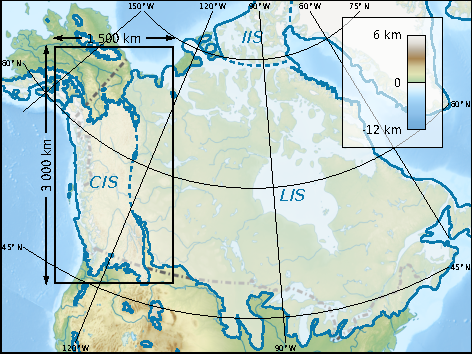
\includegraphics[width=8cm]{cordillera-climate-locmap}
	\end{center}
	\caption{Shaded relief map of northern North America with the extent of the Cordilleran (CIS), Laurentide (LIS) and Innuitian (IIS) ice sheets at 14\,$^{14}$C\,ka\,BP (16.8\,cal\,ka\,BP) \citep{dyke-2004}. While this age denotes the LIS after retreat from its LGM, it closely corresponds to the LGM extent of most of the Cordilleran ice sheet \citep{porter-swanson-1998,dyke-2004,stroeven-etal-2010}. The rectangular box denotes the modelling domain of the Cordilleran ice sheet of 1500 by 3000\,km. Major mountain ranges covered by the ice sheet include the Wrangell and St.-Elias mountains (W-SE), the Selwyn and MacKenzie mountains (S-MK), the Coast Mountains and the Rocky Mountains. The background map consists of ETOPO1 \citep{data:etopo1} and Natural Earth Data \citep{data:naturalearth} and was assembled with GRASS~GIS \citep{soft:grass}.}
	\label{fig:locmap}
\end{figure}

% fig:topo
\begin{figure*}[t]
	\vspace*{2mm}
	\begin{center}
		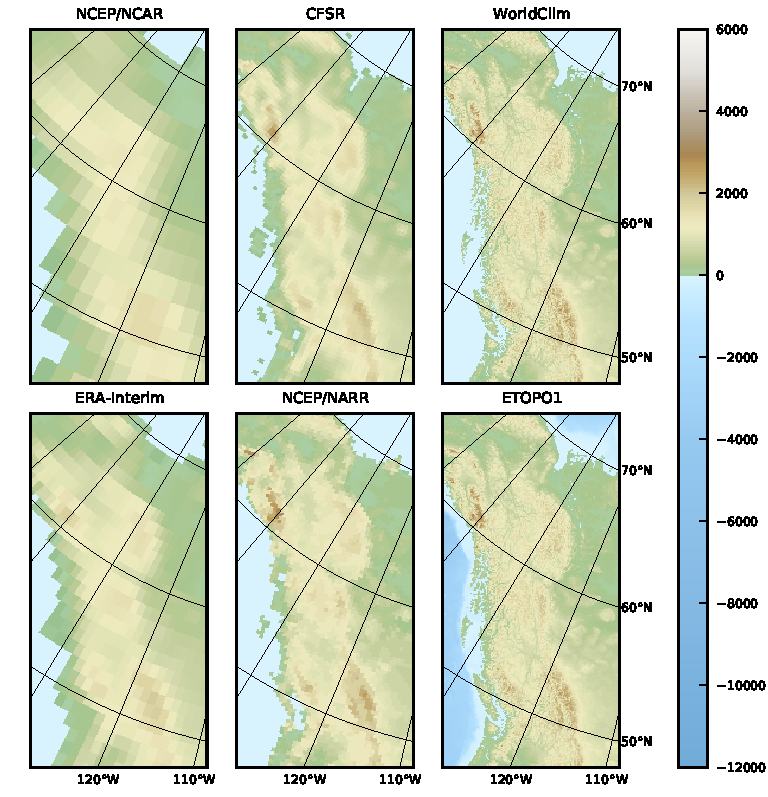
\includegraphics{cordillera-climate-topo}
	\end{center}
	\caption{Topography maps from WorldClim \citep{data:worldclim}, ERA-Interim reanalysis \citep{data:erai}, North American Regional Reanalysis \citep[NARR;][]{data:narr}, ETOPO1 \citep{data:etopo1}, Climate Forecast System Reanalysis \citep[CFSR;][]{data:cfsr}, and NCEP/NCAR reanalysis \citep{data:ncar}. Whereas ETOPO1 is used as basal topography for the ice sheet model, all other data are used as a reference for temperature lapse-rate corrections. Fig.~\ref{fig:topo}-\ref{fig:durationstack} are drawn using Matplotlib \citep{soft:mpl}.}
	\label{fig:topo}
\end{figure*}

% fig:temp
\begin{figure*}[t]
	\vspace*{2mm}
	\begin{center}
		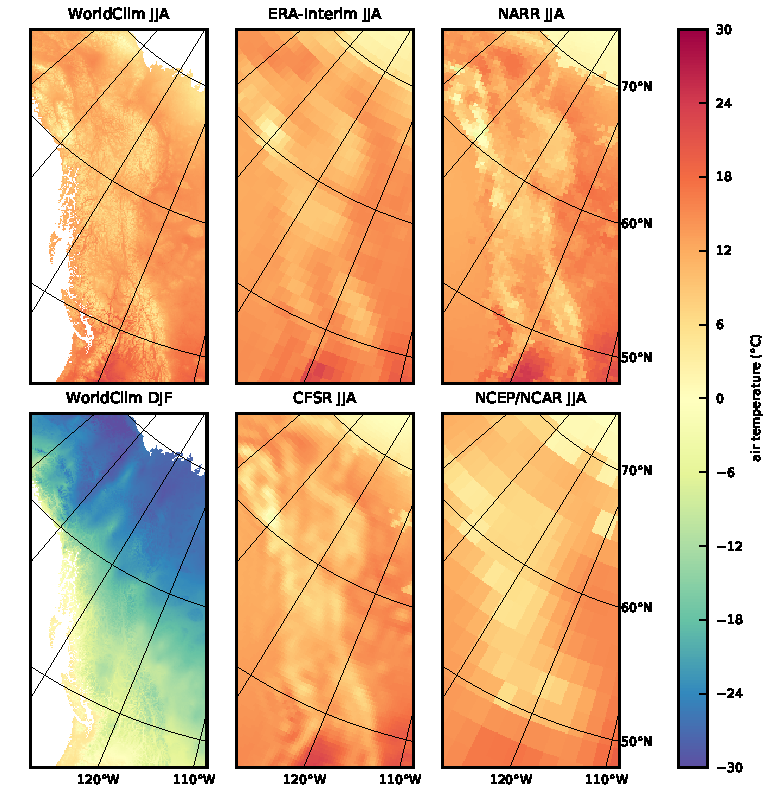
\includegraphics{cordillera-climate-temp}
	\end{center}
	\caption{Summer (JJA) and winter (DJF) temperature maps from WorldClim \citep{data:worldclim}, and summer (JJA) temperature maps from ERA-Interim reanalysis \citep{data:erai}, North American Regional Reanalysis \citep[NARR;][]{data:narr}, Climate Forecast System Reanalysis \citep[CFSR;][]{data:cfsr}, and NCEP/NCAR reanalysis \citep{data:ncar} climatologies.}
	\label{fig:temp}
\end{figure*}

% fig:prec
\begin{figure*}[t]
	\vspace*{2mm}
	\begin{center}
		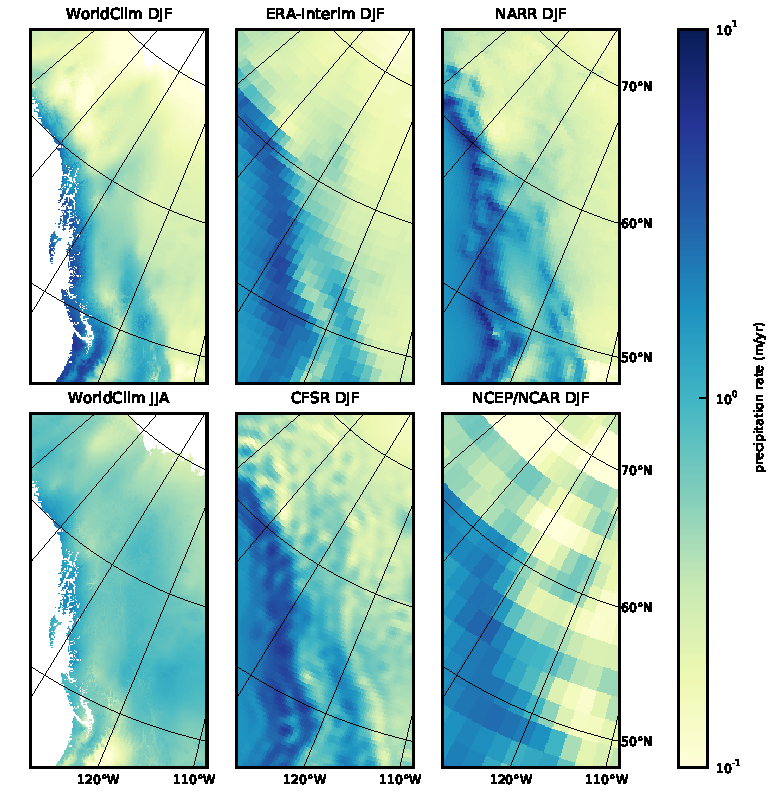
\includegraphics{cordillera-climate-prec}
	\end{center}
	\caption{Winter (DJF) and summer (JJA) precipitation maps from WorldClim \citep{data:worldclim}, and winter (DFJ) temperature maps from ERA-Interim reanalysis \citep{data:erai}, North American Regional Reanalysis \citep[NARR;][]{data:narr}, Climate Forecast System Reanalysis \citep[CFSR;][]{data:cfsr}, and NCEP/NCAR reanalysis \citep{data:ncar} climatologies. Additional forcing data was prepared to correct for wave-like precipitation artefacts in CFSR (section~\ref{sec:climate}).}
	\label{fig:prec}
\end{figure*}

% fig:ivolarea
\begin{figure}[t]
	\vspace*{2mm}
	\begin{center}
		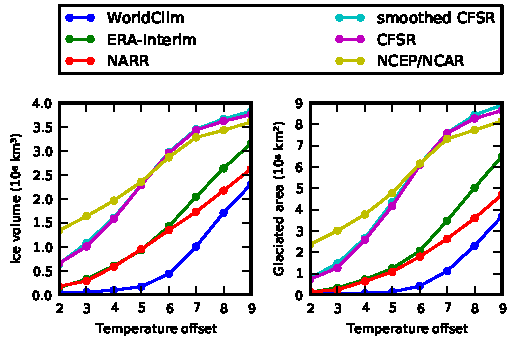
\includegraphics{cordillera-climate-ivolarea}
	\end{center}
	\caption{Total glaciated area and ice volume after 10\,ka as a function of temperature offset for each climate forcing used.}
	\label{fig:ivolarea}
\end{figure}

% fig:extent
\begin{figure*}[t]
	\vspace*{2mm}
	\begin{center}
		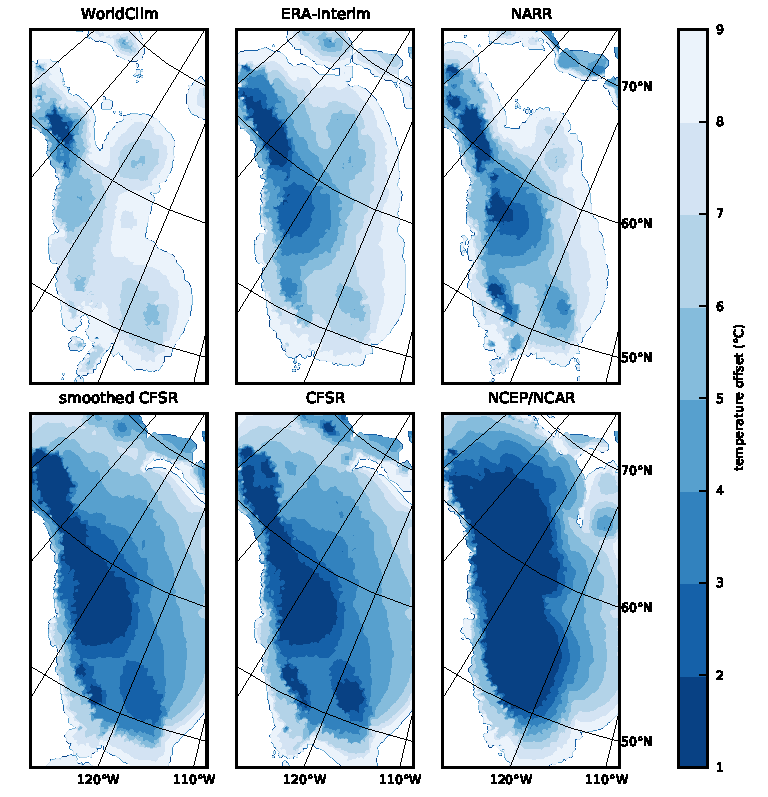
\includegraphics{cordillera-climate-extent}
	\end{center}
	\caption{Extent of ice cover after 10\,ka as a function of applied temperature offsets for each climate forcing used. A reconstructed LGM ice sheet margin by \citet{dyke-2004} (Fig.~\ref{fig:locmap}) is given for reference (black line).}
	\label{fig:extent}
\end{figure*}

% fig:cool05
\begin{figure*}[t]
	\vspace*{2mm}
	\begin{center}
		\includegraphics{cordillera-climate-cool05}
	\end{center}
	\caption{Ice surface topography (1 km contours) and velocity (\unit{m\,a^{-1}}) after 10\,ka under a climate 5\,\unit{\degree C} colder than present for each climate forcing used.}
	\label{fig:cool05}
\end{figure*}

% fig:tempheatmap
\begin{figure}[t]
	\vspace*{2mm}
	\begin{center}
		\includegraphics{cordillera-climate-tempheatmap}
	\end{center}
	\caption{Density maps showing a comparison of summer (JJA) surface air temperature data from the WorldClim climatology, against that of each reanalysis. Apparent horizontal lines are an artefact of different horizontal resolutions. Colour mapping is based on a logarythmic scale. Note the cold bias of NCEP/NCAR data relative to WorldClim data.}
	\label{fig:tempheatmap}
\end{figure}

% fig:tempdiff
\begin{figure}[t]
	\vspace*{2mm}
	\begin{center}
		\includegraphics{cordillera-climate-tempdiff}
	\end{center}
	\caption{Summer (JJA) surface air temperature difference maps against WorldClim data, after bi-linear spatial interpolation. Note the cold bias of NCEP/NCAR data and temperature anomalies due to unresolved topographic detail.}
	\label{fig:tempdiff}
\end{figure}

% fig:precheatmap
\begin{figure}[t]
	\vspace*{2mm}
	\begin{center}
		\includegraphics{cordillera-climate-precheatmap}
	\end{center}
	\caption{Density maps showing a comparison of winter (DJF) precipitation rate from the WorldClim climatology, against that of each reanalysis. Apparent horizontal lines are an artefact of different horizontal resolutions. Apparent vertical lines at low values are an artefact of the low precision of WorldClim data. Colour mapping is based on a logarythmic scale. Note the wet bias of all reanalysis data relative to WorldClim data.}
	\label{fig:precheatmap}
\end{figure}

% fig:precdiff
\begin{figure}[t]
	\vspace*{2mm}
	\begin{center}
		\includegraphics{cordillera-climate-precdiff}
	\end{center}
	\caption{Winter (DJF) precipitation rate difference maps against WorldClim data, after bi-linear spatial interpolation. Note the wet bias of all reanalysis data and the large anomalies of CFSR and NCEP/NCAR data.}
	\label{fig:precdiff}
\end{figure}

% fig:oroprecip
\begin{figure}[t]
	\vspace*{2mm}
	\begin{center}
		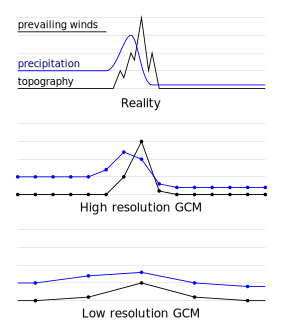
\includegraphics{cordillera-climate-oroprecip}
	\end{center}
	\caption{Schematic representation of the orographic precipitation effect over a mountain range. In a GCM of low resolution, the precipitation peak appears downwind-shifted and smoother and the precipitation shadow is less pronounced than in a high resolution GCM.}
	\label{fig:oroprecip}
\end{figure}

% fig:biatm
\begin{figure*}[t]
	\vspace*{2mm}
	\begin{center}
		\includegraphics{cordillera-climate-biatm}
	\end{center}
	\caption{Ice surface topography (1 km contours) and velocity (\unit{m\,a^{-1}}) after 10\,ka using “hybrid” climate forcing with precipitation rate from WorldClim and surface air temperature from each reanalysis (upper row), and surface air temperature from WorldClim and precipitation rate from each reanalysis (lower row). In other words, the upper row shows the effect of temperature anomalies, and the lower row the effect of precipitation anomalies, for each reanalysis, relative to WorldClim data. Each simulation uses a 5\,\unit{\degree C} offset for comparison with figure~\ref{fig:cool05}}
	\label{fig:biatm}
\end{figure*}

% fig:biatmbars
\begin{figure}[t]
	\vspace*{2mm}
	\begin{center}
		\includegraphics{cordillera-climate-biatmbars}
	\end{center}
	\caption{Effect of temperature and precipitation anomalies (separately and jointly) from each reanalysis on modelled final ice volume relative to the result of the WorldClim 5\,\unit{\degree C} offset simulation. Corresponding ice sheet geometries are presented in figures~\ref{fig:cool05} and~\ref{fig:biatm}}
	\label{fig:biatmbars}
\end{figure}

% fig:best
\begin{figure*}[t]
	\vspace*{2mm}
	\begin{center}
		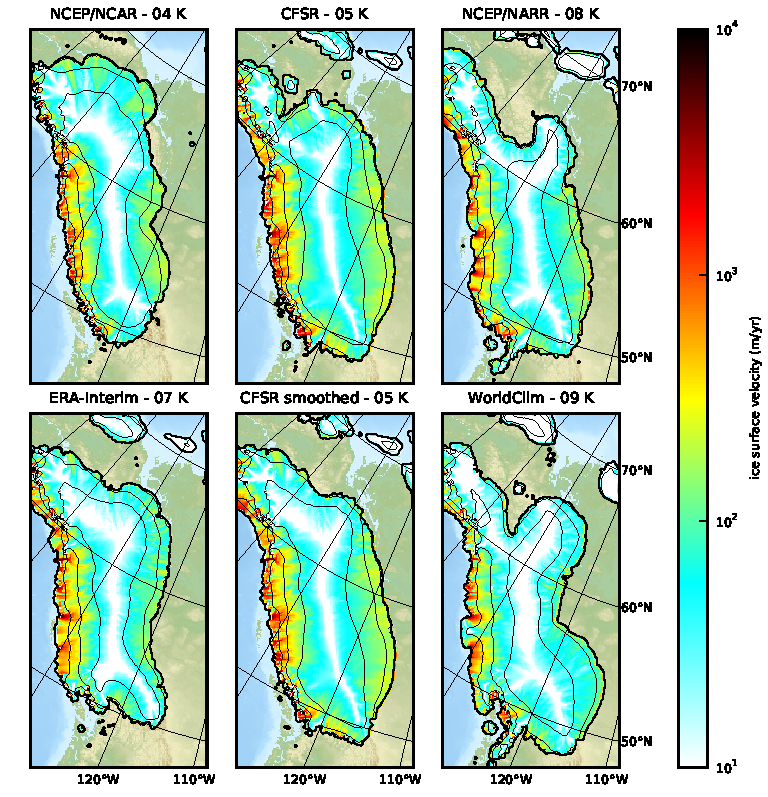
\includegraphics{cordillera-climate-best}
	\end{center}
	\caption{Ice surface topography (1\,km contours) after 10\,ka using temperature offsets resulting in glaciated areas of circa $2\,\times10^6\,\unit{km^2}$. A reconstructed LGM ice sheet margin by \citet{dyke-2004} (Fig.~\ref{fig:locmap}) is given for reference (blue line).}
	\label{fig:best}
\end{figure*}

% fig:durationstack
\begin{figure}[t]
	\vspace*{2mm}
	\begin{center}
		\includegraphics{cordillera-climate-durationstack}
	\end{center}
	\caption{Left panel: model sensitivity to simulation length. Modelled glaciated area, using NARR forcing data, and temperature offsets from 0 to 15\,\unit{\degree C}, solid lines corresponding to values from 7 to 11\,\unit{\degree C}. Right panel: modelled ice margin corresponding to temperature offsets from 7 to 11\,\unit{\degree C} when total glaciated area reach the approximate size of the LGM Cordilleran Ice Sheet of $2\,\times10^6\,\unit{km^2}$. A reconstructed LGM ice sheet margin by \citet{dyke-2004} (Fig.~\ref{fig:locmap}) is given for reference (grey shading). Note that shorter (and colder) simulations lead to more restrictive glaciation of the continental eastern margin but further ice extent in the maritime south-western part of the modelling domain.}
	\label{fig:durationstack}
\end{figure}


% ----------------------------------------------------------------------
\end{document}
% ----------------------------------------------------------------------
